\sect{Grundlagen}\label{sec:grundlagen}

\ssect{Alphabete}

Ein \textbf{Alphabet} $\Sigma$ ist eine \emph{endliche, nichtleere} Mengen von Symbolen.
\textbf{Symbole} werden häufig durch Kleinbuchstaben dargestellt.
\begin{itemize}
    \item $\Sigma = \{a, b, c\}$: Mengen von drei Symbolen
    \item $\Sigma_{\text{Bool}} = \{ 0,1 \}$: Boolesches Alphabet
    \item $\N, \R, \Z$ sind \textbf{keine} Alphabete ($\infty$ Mächtigkeit)
\end{itemize}

\ssect{Wörter}

Ein \textbf{Wort} (Zeichenreihe, String) ist eine \emph{endliche} Folge von Symbolen eines bestimmten Alphabets.
\begin{itemize}
    \item $abc$: Wort über $\Sigma_\text{lat}$ (oder $\Sigma = \{a,b,c\}$)
    \item $100111$: Wort über Alphabet ${0,1}$
    \item $\varepsilon$: Leeres Wort (über jede Alphabet)
\end{itemize}

Die \textbf{Länge eines Wortes} $w$ ist die Anzahl der Symbole und wird mit $|w|$ bezeichnet.
\begin{multicols}{2}
    \begin{itemize}
        \item $|100111| = 6$
        \item $|\varepsilon| = 0$
    \end{itemize}
\end{multicols}

$|w|_x$ bezeichnet die \textbf{absolute Häufigkeit eines Symbols $x$} in einem Wort $w$.

Mit $w^R$ wird das \textbf{Spiegelwort} zu $w$ bezeichnet.
Falls $w = w^R$, dann handelt es sich um ein \textbf{Palindrom}.

\sssect{Teilwort, Suffix und Präfix}

$v$ ist ein \textbf{Teilwort (Infix)} von $w$, wenn man $w$ als $w = xvy$ für beliebige Wörter $x$ und $y$ über $\Sigma$ schreiben kann.

Ein Wort $v$ ist ein \textbf{Präfix} von $w$, wenn $w = vy$ gilt für beliebiges Wort $y$.

Ein Wort $v$ ist ein \textbf{Suffix} von $w$, wenn $w = xv$ gilt für beliebiges Wort $x$.

Für Teilwörter, Präfixe und Suffixe von $w$ gilt: Sie sind \textbf{echt}, falls sie nicht gleich $w$.

\ssect{Sprachen}

Eine Teilmenge $L \subseteq \Sigma^*$ von Wörtern über einem Alphabet $\Sigma$ wird als \textbf{Sprache über $\Sigma$} bezeichnet.
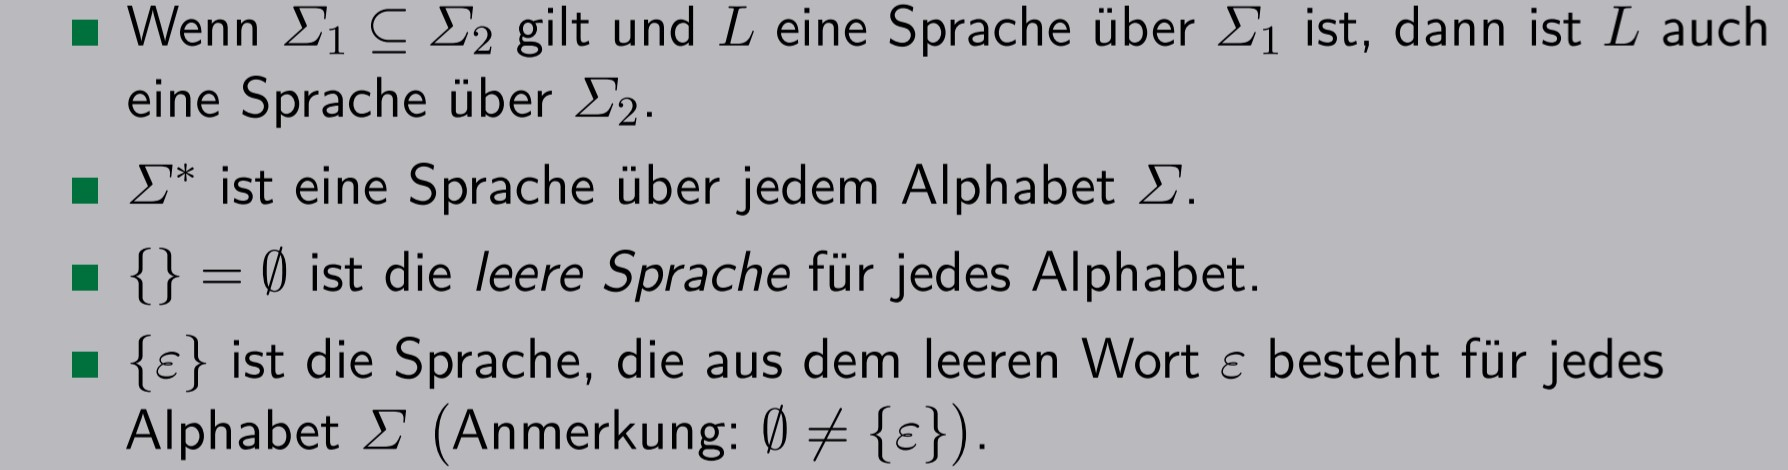
\includegraphics[scale=0.14]{sprache}

\textbf{Menge von Wörter}
{\fontsize{6}{7}
    \begin{itemize}
        \item $\Sigma^* = \underbrace{\Sigma^0}_{1} \cup \underbrace{\Sigma^1}_2 \cup \underbrace{\Sigma^2}_4 \cup \dots$ (Kleensche Hülle)
        \item $\Sigma^+ = \underbrace{\Sigma^1}_2 \cup \underbrace{\Sigma^2}_4 \cup \underbrace{\Sigma^3}_8 \dots = \Sigma^* \backslash \{ \varepsilon \}$ (Pos.\ Hülle)
    \end{itemize}
}

\textbf{Konkatenation:} Verkettung von zwei beliebigen Wörtern $x$ und $y$ \[x \circ y = xy \coloneqq (x_1, x_2, \dots, x_n, y_1, y_2, \dots, y_m)\]
\textbf{Wortpotenzen:}
\begin{itemize}
    \item $x^{n+1} = x^n \circ x = x^n x$
    \item $bbababababbaaaabab = b^2 (ab)^4 ba^3 (ab)^2$
\end{itemize}